\section{単一粒子の非相対論的な量子力学}

\noindent\textbf{この章の中心命題}
\[
\boxed{
i\hbar\frac{\partial}{\partial t}\psi(\mathbf{x},t)
=
\left(
-\frac{\hbar^2}{2m}\nabla^2+V(\mathbf{x})
\right)\psi(\mathbf{x},t)
}
\]
ポテンシャルと境界条件を与えると、この方程式が許される波動関数とエネルギー固有値を決める。

\subsection{シュレーディンガー方程式の導出}
単一粒子の非相対論的理論では、まず「古典極限では粒子のエネルギー関係に戻り、同時に波としての振る舞いを記述する」時間発展方程式を求めたい。出発点は、古典力学における粒子のエネルギーと運動量の関係
\begin{equation}
    E = \frac{\mathbf{p}^2}{2m} + V(\mathbf{x})
\end{equation}
である。一方、光については黒体放射と光電効果の解析から、振動数 $\nu$ の光がエネルギー $h\nu$ をもつ量子として振る舞うことが分かり、さらにコンプトン効果などから運動量も
\[
E = h\nu,\qquad p=\frac{h}{\lambda}
\]
が成り立つことが分かっていた。ド・ブロイはこの関係を物質粒子にも拡張し、角振動数 $\omega=2\pi\nu$ と波数 $\mathbf{k}$ を用いて
\[
E = \hbar \omega,\qquad \mathbf{p} = \hbar \mathbf{k}
\]
を仮定した。そこで粒子の状態を複素振幅 $\psi(\mathbf{x},t)$ で表す。観測で直接得られるのは、各試行で粒子がどこに検出されたかという統計である。二重スリット実験が示すように、その統計分布は振幅の重ね合わせによって決まり、したがって基本量は確率そのものではなく干渉する複素振幅でなければならない。ボルンは、その絶対値の二乗
\[
|\psi(\mathbf{x},t)|^2
\]
を位置の確率密度と読むべきだと提案した。
全確率が有限で
\[
\int_{\mathbb{R}^3} |\psi(\mathbf{x},t)|^2\,d^3x < \infty
\]
であることを要求すると、固定時刻での状態空間として
\[
\mathcal{H}_1 := L^2(\mathbb{R}^3,d^3x)
\]
を固定時刻の状態空間として選ぶ。これは、内積
\[
\langle \psi,\varphi\rangle
:=
\int_{\mathbb{R}^3}\psi(\mathbf{x})^*\varphi(\mathbf{x})\,d^3x
\]
によって全確率 $\|\psi\|^2$ を表せる空間だからである。

まず、波数 $\mathbf{k}$ と角振動数 $\omega$ をもつ平面波
\[
\psi(\mathbf{x}, t) = e^{i(\mathbf{k} \cdot \mathbf{x} - \omega t)}
\]
を考える。これは厳密には $L^2(\mathbb{R}^3)$ の元ではないが、一般の波束をフーリエ積分で記述するときの基本成分になっている。実際、波束は平面波の重ね合わせ
\[
\psi(\mathbf{x},t)
=
\int \frac{d^3k}{(2\pi)^3}\,\tilde{\psi}(\mathbf{k})e^{i(\mathbf{k}\cdot \mathbf{x}-\omega t)}
\]
として表される。したがって、平面波に対して成り立つ微分作用素の関係式は、重ね合わせによって一般の波束にも引き継がれる。平面波に時間微分および空間微分を作用させると、
\begin{equation}
    i\hbar \frac{\partial}{\partial t} \psi = \hbar \omega \psi = E \psi, \quad -i\hbar \nabla \psi = \hbar \mathbf{k} \psi = \mathbf{p} \psi
\end{equation}
が成り立つ。したがって、エネルギーと運動量にはそれぞれ
\begin{equation}
    \hat{E} = i\hbar \frac{\partial}{\partial t}, \quad \hat{\mathbf{p}} = -i\hbar \nabla
\end{equation}
という演算子を対応させる。ここでは、平面波に対する固有値が実験的な関係 $E=\hbar\omega,\mathbf{p}=\hbar\mathbf{k}$ と一致することを対応の条件としている。これが対応原理である。

そこで、先ほどの古典的関係にこれらの演算子を代入すると、時間発展を定める方程式としてシュレーディンガー方程式
\begin{equation}
    i\hbar \frac{\partial}{\partial t} \psi = \left( -\frac{\hbar^2}{2m} \nabla^2 + \hat{V}(\mathbf{x}) \right) \psi = \hat{H} \psi
\end{equation}
が得られる。すなわち、古典的なエネルギー保存則を波動関数に作用する演算子の関係へと読み替えることで、量子力学の基本方程式が導かれる。これは線形な微分方程式であり、二つの解 $\psi_1,\psi_2$ に対して $a\psi_1+b\psi_2$ も解になるため、重ね合わせの原理と両立する。

シュレーディンガー方程式の重要な役割は、ポテンシャルと境界条件を与えたときに、許される状態とエネルギー固有値を具体的に決める点にある。典型的な例を三つ挙げる。
\subsection{シュレーディンガー方程式の基本的な解}
\paragraph{無限深井戸}
一次元で
\[
V(x)=
\begin{cases}
0 & (0 < x < L) \\
\infty & (\text{otherwise})
\end{cases}
\]
とする。壁の外では波動関数が消えなければならないため、定常状態 $\psi(x,t)=\phi(x)e^{-iEt/\hbar}$ の空間部分は
\[
\phi_n(x)=\sqrt{\frac{2}{L}}\sin\frac{n\pi x}{L}, \quad E_n=\frac{\hbar^2\pi^2 n^2}{2mL^2}\qquad(n=1,2,\dots)
\]
となる。これは次のように求まる。井戸の内部では $V(x)=0$ であるから、定常状態 $\psi(x,t)=\phi(x)e^{-iEt/\hbar}$ に対して
\[
-\frac{\hbar^2}{2m}\frac{d^2\phi}{dx^2}=E\phi
\]
である。ここで
\[
k^2:=\frac{2mE}{\hbar^2}
\]
とおけば一般解は
\[
\phi(x)=A\sin kx+B\cos kx
\]
となる。無限壁のため境界条件は
\[
\phi(0)=0,\qquad \phi(L)=0
\]
であり、最初の条件から $B=0$、二つ目の条件から
\[
\sin kL=0
\qquad\Longrightarrow\qquad
k=\frac{n\pi}{L}\qquad(n=1,2,\dots)
\]
を得る。したがって
\[
E_n=\frac{\hbar^2k^2}{2m}=\frac{\hbar^2\pi^2n^2}{2mL^2}
\]
となり、さらに正規化条件
\[
\int_0^L |\phi_n(x)|^2\,dx = 1
\]
から
\[
\phi_n(x)=\sqrt{\frac{2}{L}}\sin\frac{n\pi x}{L}
\]
が従う。境界条件だけでエネルギーが離散化されることが分かる。

\paragraph{有限ポテンシャル障壁}
たとえば
\[
V(x)=
\begin{cases}
V_0 & (0 < x < L) \\
0 & (\text{otherwise})
\end{cases}
\]
という障壁を考える。古典力学では、粒子のエネルギーが $E<V_0$ なら粒子は障壁を越えられず、透過確率は $0$ である。しかし量子力学では、左から粒子が入射する状況を
\[
\psi_I(x)=e^{ikx}+r e^{-ikx}\qquad (x<0),
\]
\[
\psi_{II}(x)=A e^{\kappa x}+B e^{-\kappa x}\qquad (0<x<L),
\]
\[
\psi_{III}(x)=t e^{ikx}\qquad (x>L)
\]
と書ける。ここで
\[
k=\frac{\sqrt{2mE}}{\hbar},\qquad
\kappa=\frac{\sqrt{2m(V_0-E)}}{\hbar}
\]
である。$\psi$ と $d\psi/dx$ の連続条件を $x=0,L$ で課す。透過係数を求めるための連立方程式は
\[
1+r=A+B,
\qquad
ik(1-r)=\kappa(A-B),
\]
\[
Ae^{\kappa L}+Be^{-\kappa L}=te^{ikL},
\qquad
\kappa(Ae^{\kappa L}-Be^{-\kappa L})=ikte^{ikL}
\]
という4本の方程式から決まる。まず $x=L$ の二式から
\[
Ae^{\kappa L}
=
\frac{te^{ikL}}{2}\left(1+\frac{ik}{\kappa}\right),
\qquad
Be^{-\kappa L}
=
\frac{te^{ikL}}{2}\left(1-\frac{ik}{\kappa}\right)
\]
を得る。これを $x=0$ の二式に代入すると、
\[
1+r
=
te^{ikL}
\left(
\cosh\kappa L-\frac{ik}{\kappa}\sinh\kappa L
\right),
\]
\[
1-r
=
te^{ikL}
\left(
\cosh\kappa L+\frac{i\kappa}{k}\sinh\kappa L
\right)
\]
となる。二式を足して $r$ を消去すれば
\[
t
=
\frac{2e^{-ikL}}
{2\cosh\kappa L
+i\left(\frac{\kappa}{k}-\frac{k}{\kappa}\right)\sinh\kappa L}
\]
である。したがって
\[
|t|^2
=
\left[
1+\frac{1}{4}
\left(\frac{\kappa}{k}+\frac{k}{\kappa}\right)^2
\sinh^2(\kappa L)
\right]^{-1}
\]
となる。ここで
\[
\left(\frac{\kappa}{k}+\frac{k}{\kappa}\right)^2
=
\frac{(\kappa^2+k^2)^2}{\kappa^2k^2}
=
\frac{V_0^2}{E(V_0-E)}
\]
を用いると、透過係数は
\[
T:=|t|^2
=
\left[
1+\frac{V_0^2}{4E(V_0-E)}\sinh^2(\kappa L)
\right]^{-1}
\]
となる。右辺は有限な $L$ に対して正であるから、
\[
E<V_0 \quad\Longrightarrow\quad T>0
\]
である。すなわち、障壁内部で波動関数が指数関数的に減衰しながらも消えず、その結果として古典力学では禁じられていた透過が起こる。これがトンネル効果である。
図~\ref{fig:tunneling} はこの状況の模式図である。障壁内部では振幅が指数関数的に小さくなるが、有限の幅 $L$ をもつ限り右側へ抜けた成分が残る。

\begin{figure}[t]
\centering
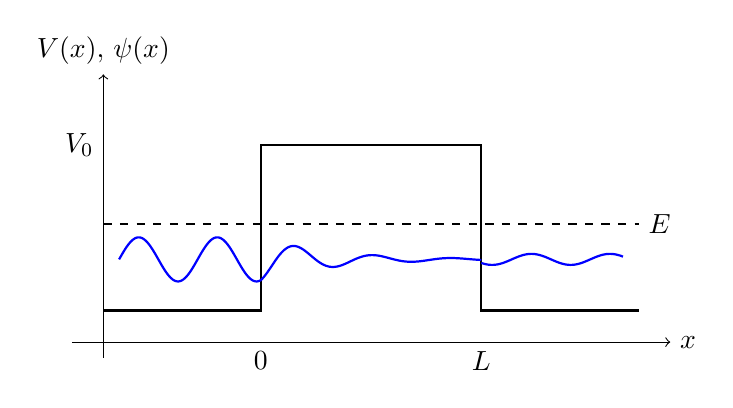
\begin{tikzpicture}[x=1cm,y=1cm]
    \draw[->] (-0.4,0) -- (7.2,0) node[right] {$x$};
    \draw[->] (0,-0.2) -- (0,3.4) node[above] {$V(x),\,\psi(x)$};

    \draw[thick] (0,0.4) -- (2.0,0.4) -- (2.0,2.5) -- (4.8,2.5) -- (4.8,0.4) -- (6.8,0.4);
    \draw[dashed] (0,1.5) -- (6.8,1.5);

    \node[left] at (0,2.5) {$V_0$};
    \node[right] at (6.8,1.5) {$E$};
    \node[below] at (2.0,0) {$0$};
    \node[below] at (4.8,0) {$L$};

    \draw[blue,thick,samples=120,domain=0.2:2.0,smooth]
        plot (\x,{1.05 + 0.28*sin(deg(6.3*(\x-0.2)))});
    \draw[blue,thick,samples=140,domain=2.0:4.8,smooth]
        plot (\x,{1.05 + 0.28*exp(-1.15*(\x-2.0))*sin(deg(6.3*(\x-0.2)))});
    \draw[blue,thick,samples=120,domain=4.8:6.6,smooth]
        plot (\x,{1.05 + 0.07*sin(deg(6.3*(\x-0.2)))});
\end{tikzpicture}
\caption{有限ポテンシャル障壁に対するトンネル効果の模式図。古典力学では $E<V_0$ の粒子は障壁を越えられないが、量子力学では障壁内部で波動関数が減衰しつつ、右側にも有限の透過振幅が残る。}
\label{fig:tunneling}
\end{figure}
\paragraph{調和振動子}
ポテンシャル
\[
V(x)=\frac{1}{2}m\omega^2 x^2
\]
をもつ調和振動子では、生成・消滅演算子
\[
\hat{a}
:=
\sqrt{\frac{m\omega}{2\hbar}}
\left(
\hat{x}+\frac{i}{m\omega}\hat{p}
\right),
\qquad
\hat{a}^\dagger
:=
\sqrt{\frac{m\omega}{2\hbar}}
\left(
\hat{x}-\frac{i}{m\omega}\hat{p}
\right)
\]
を導入すると、
\[
[\hat{a},\hat{a}^\dagger]=1
\]
が成り立つ。ハミルトニアン
\[
\hat{H}
=
\frac{\hat{p}^2}{2m}+\frac{1}{2}m\omega^2\hat{x}^2
\]
は
\[
\hat{H}=\hbar\omega\left(\hat{a}^\dagger \hat{a}+\frac{1}{2}\right)
\]
と書ける。ここで
\[
\hat{N}:=\hat{a}^\dagger \hat{a}
\]
とおく。$\hat{N}$ の固有値を求めるため、交換関係から
\[
[\hat{N},\hat{a}^\dagger]=\hat{a}^\dagger,
\qquad
[\hat{N},\hat{a}]=-\hat{a}
\]
が従うことを使う。もし
\[
\hat{N}|n\rangle=n|n\rangle
\]
なら、
\[
\hat{N}\hat{a}^\dagger|n\rangle
=
(n+1)\hat{a}^\dagger|n\rangle,
\qquad
\hat{N}\hat{a}|n\rangle
=
(n-1)\hat{a}|n\rangle
\]
である。すなわち、$\hat{a}^\dagger$ は $\hat{N}$ の固有値を1だけ上げ、$\hat{a}$ は1だけ下げる。また
\[
\langle n|\hat{N}|n\rangle
=
\|\hat{a}|n\rangle\|^2
\ge 0
\]
であるから、固有値は負にはなれない。したがって降下操作はどこかで止まり、最低状態 $|0\rangle$ は
\[
\hat{a}|0\rangle=0,
\qquad
\hat{N}|0\rangle=0
\]
を満たす。そこから $\hat{a}^\dagger$ を繰り返し作用させることで
\[
|n\rangle\propto(\hat{a}^\dagger)^n|0\rangle,
\qquad
n=0,1,2,\dots
\]
が得られる。ゆえに $\hat{N}$ の固有値は $n=0,1,2,\dots$ であり、エネルギー固有値は
\[
E_n = \hbar \omega \left(n + \frac{1}{2}\right)
\]
となる。とくに基底状態 $|0\rangle$ は
\[
\hat{a}|0\rangle = 0
\]
で定まり、そのエネルギーは
\[
E_0=\frac{\hbar\omega}{2}
\]
である。基底状態のエネルギーが $0$ ではなく $\hbar\omega/2$ だけ残る点は、量子揺らぎの典型例である。

\subsubsection*{対称性・ネーターの定理と生成子}
交換関係に入る前に、古典力学で対称性と保存量がどのように結び付いているかを確認しておく。ラグランジアン $L(q,\dot q,t)$ が無限小変換
\[
q_i \mapsto q_i + \varepsilon \Delta q_i,
\qquad
t \mapsto t + \varepsilon \Delta t
\]
の下で全微分を除いて不変、すなわち
\[
\delta L = \varepsilon \frac{dF}{dt}
\]
となるとき、ネーターの定理により
\[
Q = \sum_i p_i \Delta q_i - H\Delta t - F,
\qquad
p_i := \frac{\partial L}{\partial \dot q_i}
\]
は保存される。ここで $p_i$ は共役運動量、$H:=\sum_i p_i\dot q_i-L$ はハミルトニアンである。代表的な対応は
\[
t \mapsto t+\varepsilon, \qquad
\mathbf{x} \mapsto \mathbf{x}+\mathbf{a}, \qquad
\mathbf{x} \mapsto \mathbf{x}+\boldsymbol{\theta}\times \mathbf{x}
\]
\[
\Longleftrightarrow
\qquad
H,\qquad \mathbf{P},\qquad \mathbf{J}
\]
であり、それぞれ時間並進、空間並進、空間回転に対する生成子が、エネルギー、運動量、角運動量になっている。

ハミルトン形式では、保存量は単に「保存される量」であるだけでなく、その対称変換を生み出す生成子として働く。古典力学では、無限小変換はポアソン括弧を用いて
\[
\delta A = \varepsilon \{A, G\}
\]
と書ける。ここで $G$ が生成子、$\varepsilon$ が無限小の変換パラメータである。たとえば空間並進では $G=p$ であり、
\[
\delta x = \varepsilon \{x,p\} = \varepsilon
\]
となるから、運動量 $p$ が位置を平行移動させる生成子であることが分かる。同様に、時間並進の生成子はハミルトニアン $H$ であり、回転の生成子は角運動量 $L$ である。

量子力学では、この構造が交換関係へと引き継がれる。対称変換は状態の内積、したがって遷移確率を保たなければならないから、連続対称性はユニタリ演算子で表される。単位変換の近くで連続につながる一パラメータ変換は
\[
\hat{U}(\varepsilon)=\exp\!\left(-\frac{i}{\hbar}\varepsilon \hat{G}\right)
\]
と書ける。これを $\varepsilon$ について展開すると無限小変換は
\[
\hat{U}(\varepsilon)^\dagger \hat{A} \hat{U}(\varepsilon)
= \hat{A} + \frac{i\varepsilon}{\hbar}[\hat{G},\hat{A}] + O(\varepsilon^2)
\]
となる。したがって、古典力学の
\[
\delta A = \varepsilon\{A,G\}
\]
に対応する量として、量子力学では
\[
\delta \hat{A} = \frac{i\varepsilon}{\hbar}[\hat{G},\hat{A}]
\]
が現れる。

\subsection{交換関係とその意義}
とくに空間並進の生成子が運動量であることを量子論で表すと、位置演算子 $\hat{x}$ は
\[
\hat{U}(a)^\dagger \hat{x}\hat{U}(a)=\hat{x}+a
\]
と変換しなければならず、これが正準交換関係
\[
[\hat{x},\hat{p}]=i\hbar
\]
を導く。つまり交換関係は、古典力学における生成子とポアソン括弧の構造を量子論へ持ち込んだものと見なせる。
実際、位置表示では $\hat{x}=x$, $\hat{p}=-i\hbar \frac{d}{dx}$ であるから、任意の波動関数 $\psi(x)$ に対して
\[
[\hat{x},\hat{p}]\psi(x)
= x\left(-i\hbar \frac{d\psi}{dx}\right) + i\hbar \frac{d}{dx}(x\psi(x))
= i\hbar \psi(x)
\]
となり、交換関係が確かめられる。

この関係の意義は、位置と運動量が同時に鋭く定まる共通固有状態を持たないという点にある。さらに、運動量が空間並進の生成子であること、後に述べる不確定性原理、そしてハイゼンベルク方程式の構造は、いずれもこの交換関係に支えられている。

\subsection{不確定性原理}
状態 $\psi$ における物理量 $\hat{A}$ の期待値を $\langle \hat{A} \rangle$ とし、
\[
\Delta \hat{x} := \hat{x} - \langle \hat{x} \rangle, \quad \Delta \hat{p} := \hat{p} - \langle \hat{p} \rangle
\]
とおく。標準偏差は
\[
(\Delta x)^2 = \langle (\Delta \hat{x})^2 \rangle, \quad (\Delta p)^2 = \langle (\Delta \hat{p})^2 \rangle
\]
で与えられる。ここで、ベクトル $\Delta \hat{x}\psi$ と $\Delta \hat{p}\psi$ にコーシー--シュワルツの不等式を適用すると、
\[
(\Delta x)^2(\Delta p)^2 \ge \left| \langle \Delta \hat{x}\Delta \hat{p} \rangle \right|^2
\]
を得る。さらに、複素数 $z$ に対して $|z| \ge |\operatorname{Im} z|$ であることと、
\[
\operatorname{Im}\langle \Delta \hat{x}\Delta \hat{p} \rangle
= \frac{1}{2i}\langle [\Delta \hat{x}, \Delta \hat{p}] \rangle
= \frac{1}{2i}\langle [\hat{x}, \hat{p}] \rangle
= \frac{\hbar}{2}
\]
を用いれば、
\[
\Delta x \, \Delta p \ge \frac{\hbar}{2}
\]
が従う。したがって、不確定性原理は測定器の不完全さではなく、交換関係そのものから出てくる量子論の構造的な制約である。

ここまでで、非相対論的一粒子量子力学の基本構造はそろった。次節では、同じ理論を状態ベクトルではなく演算子の時間発展を前面に出すハイゼンベルク描像で書き直す。
